\chapter{若当标准形}
在之前的叙述中我们说明了复向量空间中算子都有分块对角矩阵,且每个分块都具有上三角矩阵的形式.本节我们希望每个分块能获得
比上三角矩阵更多0的形式.实际上,这一形式我们之前已经引入,并且也讨论了其极小多项式,本节中我们讨论如何得到这种形式的
矩阵,了解算子和矩阵若当标准形的求法以及若当标准形对应基的求法,并讲解其应用.

\section{若当标准形的存在与形式}
在\autoref{thm:16:广义本征性质} (5) 中我们提到过$T-\lambda_jI$限制在$\lambda_j$对应的广义本征空间上是幂零算子.
因此我们可以先研究幂零算子的若当标准形,然后加入简单的数量矩阵即可.

我们仍然沿着 Done Right 的思路,尽管本节的定理证明有一种看了几行就没兴趣再看下去的美感.我们需要注意的是,Done Right 以及其它
高等代数教材中关于若当的推导都十分繁杂,因此这并不是我们考虑的重点(当然建议读者阅读证明过程以加强理解).我们的核心在于掌握
这些结论并且能够计算出若当标准形,并运用若当标准形解决一些问题.在意推导的读者可以考虑学习抽象代数,运用模论推导若当标准形,
更加直接.
\begin{theorem} \label{thm:18:若当基存在}
    设$N\in \mathcal{L}(V)$是幂零的,则存在向量$v_1,\ldots,v_n$和非负整数$m_1,\ldots,m_n$使得
    \begin{enumerate}
        \item $N^{m_1}v_1,\ldots,Nv_1,v_1,\ldots,N^{m_n}v_n,\ldots,Nv_n,v_n$是$V$的基;

        \item $N^{m_1+1}v_1=\cdots=N^{m_n+1}v_n=0$.
    \end{enumerate}
\end{theorem}
1 中的向量组可以分为$n$个由$v_i\enspace(i=1,\ldots,n)$生成的$N$-强循环子空间,即$N^{m_i}v_i,\ldots,Nv_i,v_i$.
实际上,1 中的向量排列顺序以及2中的等于0的条件的目的都是使得$N$在这组基下的表示矩阵为分块对角矩阵,
每一块的大小为$(m_i+1)\times(m_i+1)$,形如\[\begin{pmatrix}
    0 & 1 &  & 0 \\  & \ddots & \ddots &  \\  &  &  \ddots & 1 \\ 0 &  &  & 0
\end{pmatrix}\]即为若当块$J_{m_i+1}(0)$.

我们更进一步,将数量矩阵代回.由于上述若当块是$(T-\lambda_iI)\vert_{G(\lambda_i,T)}$的若当标准形,是在\autoref{thm:18:若当基存在}
中的基下的矩阵,而我们知道,$\lambda_iI$在任意一组基下的矩阵都是对角线元素均为$\lambda_j$的对角矩阵,因此我们可以得到以下结论:
\begin{theorem}
    设$T\in \mathcal{L}(V)$,则$T$在\autoref{thm:18:若当基存在} 给出的基下的矩阵表示为分块对角矩阵,且每个对角块都是
    $(m_i+1)\times(m_i+1)\enspace(i=1,\ldots,n)$的矩阵,且具有形式\[\begin{pmatrix}
        \lambda_i & 1 &  & 0 \\  & \ddots & \ddots &  \\  &  &  \ddots & 1 \\ 0 &  &  & \lambda_i
    \end{pmatrix}\]而整体的分块对角矩阵即为若当形矩阵.
\end{theorem}

接下来我们需要描述矩阵的若当标准形.实际上,算子在某组基下有若当标准形与矩阵有相似标准形为若当标准形是等价的.我们考虑$P^{-1}AP=J$,
其中$P$为过渡矩阵,$J$为$A$的若当标准形.我们可以将$A$视为$T(\alpha)=A\alpha$在自然基下的矩阵,于是$T$在\autoref{thm:18:若当基存在}
给出的基(记为$B$)下的表示矩阵的求解方式就是$T(B)=(B)J$,将$B$组成的矩阵记作$P$,由$T$的定义可知,$T(B)=(B)J$等同于$AP=PJ$,即
$P^{-1}AP=J$,故如果我们要求矩阵相似于其若当标准形的过渡矩阵,问题转化为求解若当基然后排列成矩阵即可.于是我们下面将要介绍如何将基和
若当标准形具体地求出来.

\section{若当标准形的求解}
在上一小节的最后,我们将求解若当标准形的目标转化为了求解若当基,我们希望有更加算法化的方式去实现这一目标.为此,我们先引入一些记号.
我们记$G_j(\lambda,T)=\ker (T-\lambda I)^j$,根据零空间增长以及极小多项式的结论,我们知道当$i<j$时有
$G_i(\lambda,T)\subseteq G_j(\lambda,T)$,并且当$T-\lambda I$的次数为极小多项式中该本征值对应因式的次数后,零空间会停止增长.

我们可以优先考虑幂零算子$N\in \mathcal{L}(V)$,最后再考虑非幂零的情况应当给我们的算法加什么样的步骤.我们的目标是求出一组基形如
$N^{m_1}v_1,\ldots,Nv_1,v_1,\ldots,N^{m_n}v_n,\ldots,Nv_n,v_n$,这里有两组未知量,我们依次来说明如何求解.在求解之前,我们需要引入一个
定理表明下述方法的合理性:
\begin{theorem}
    设$T\in \mathcal{L}(V)$,若$V$中向量$v\in G_j(\lambda,T)\backslash G_{j-1}(\lambda,T)$,则
    \begin{enumerate}
        \item 对任意的$i<j$,有$(T-\lambda I)^iv\in G_{j-i}(\lambda,T)\backslash G_{j-i-1}(\lambda,T)$;

        \item $v,(T-\lambda I)v,\ldots,(T-\lambda I)^{j-1}v$线性无关.
    \end{enumerate}
\end{theorem}
定理的证明是基本的,我们留作习题.这一定理对于下述算法中若当基的阶梯形排列的合理性是必要的.
\begin{enumerate}
    \item \textbf{\heiti 求解 $m_1,\ldots,m_n$}

    我们首先确定幂次参数,这一参数确定后若当形矩阵就确定了,因为若当形矩阵中每个若当块的大小是$(m_i+1)\times(m_i+1)(i=1,\cdots,n)$.
    \begin{enumerate}
        \item 我们假设$m_1\geqslant\cdots\geqslant m_n$,并在接下来的步骤中尝试将若当基重排成如图格式:

        \begin{figure}[h]
            \centering
            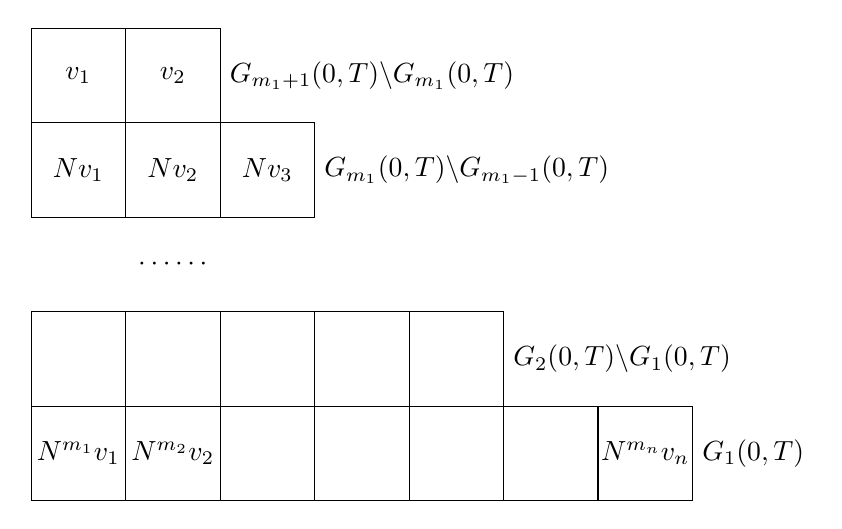
\begin{tikzpicture}
                \foreach[count=\i] \len in {2, 3, 3, 5, 7, 7}
                    \draw (0, -1.2*\i+1.2) -- (1.2*\len, -1.2*\i+1.2);

                \foreach \i in {0,...,2}
                    \draw (1.2*\i, 0) -- (1.2*\i, -2.4);
                \draw (3.6, -1.2) -- (3.6, -2.4);

                \foreach \i in {0,...,5}
                    \draw (1.2*\i, -3.6) -- (1.2*\i, -6.0);
                \foreach \i in {6,...,7}
                    \draw (1.2*\i, -4.8) -- (1.2*\i, -6.0);

                \foreach \i in {1,...,2} {
                    \node at (1.2*\i-0.6, -0.6) {$v_{\i}$};
                    \node at (1.2*\i-0.6, -5.4) {$N^{m_{\i}}v_{\i}$};
                }
                \foreach \i in {1,...,3}
                    \node at (1.2*\i-0.6, -1.8) { $Nv_{\i}$};
                \node at (7.8, -5.4) { $N^{m_n}v_n$};
                \node at (1.8, -3.0) {$\cdots\cdots$};

                \node[anchor=west] at (2.4, -0.6) {$G_{m_1+1}(0,T) \backslash G_{m_1}(0,T)$};
                \node[anchor=west] at (3.6, -1.8) {$G_{m_1}(0,T) \backslash G_{m_1-1}(0,T)$};
                \node[anchor=west] at (6.0, -4.2) {$G_2(0,T) \backslash G_1(0,T)$};
                \node[anchor=west] at (8.4, -5.4) {$G_1(0,T)$};
            \end{tikzpicture}
        \end{figure}

        即第一排将若当基中在$G_1(0,T)$的向量排列,即在$N$作用一次后就等于0的向量;第二排将所有若当基中在
        $G_2(0,T)\backslash G_1(0,T)$的向量排列,即在$N$作用一次后不等于0但作用两次等于0的向量,以此类推.
        由于假设$m_1\geqslant\cdots\geqslant m_n$,这个图呈阶梯形.
        \item 接下来要将上图填满,首先要确定求解$G_j(0,T)$及其维数(因为幂零算子本征值为0)直到
        $j$等于$N$极小多项式的次数(即幂零指数,或当$G_j(0,T)=V$时),因为此后零空间不可能继续增加,阶梯形
        也就不会再延伸.在求出维数后阶梯形状也即确定,因为各层向量个数确定了.例如假设11维空间中的映射满足
        $G_1(0,T)$,$G_2(0,T)$,$G_3(0,T)$的维数分别为5,9,11.这说明从底至上向量个数依次为5,4($=9-5$),2($=11-9$).
        \item 基于上面的求解,这时我们就可以确定若当块的阶数$m_i+1\enspace(i=1,\ldots,n)$,因为这一阶梯中第$i$列的高度实际上
        就是$m_i+1$(因为每一列是$v_i,Nv_i,\ldots,N^{m_i}v_i$).将这些若当块拼起来就得到了幂零算子的若当标准形.
    \end{enumerate}
    \item \textbf{\heiti 求解 $v_1,\ldots,v_n$}

    本节内容按照以往的情况在考试中不要求,但为了保证讲义的完整性,我们将求若当基的方法也进行描述.
    \begin{enumerate}[label=(\arabic*)]
        \item 我们在前述内容中求出了各个$G_j(0,T)$,接下来我们需要利用这些向量将之前确定形状的阶梯内容填满.
        我们首先将阶梯最上方的向量确定,实际上就是利用求出的$G_{m_1+1}(0,T)$(也就是$V$)和$G_{m_1}(0,T)$求出
        二者之差.似乎很简单,但若仔细思索便会发现线性空间的差并不一定好求.举一个简单的例子,设
        $G_{m_1+1}(0,T)=\{\alpha_1,\alpha_2,\alpha_3,\alpha_4\}$,$G_{m_1}(0,T)=\{\beta_1,\beta_2\}$.
        这其中出现的所有向量可能都完全不一样,所以作差并不容易.但我们有一种好方法,如果我们每次从$G_{m_1+1}(0,T)$
        中挑选两个向量和$G_{m_1}(0,T)$中的两个向量放在一起,如果这四个向量线性无关,这就说明这两个挑出的向量就是作差的结果.
        原因在于这相当于$G_{m_1}(0,T)$直和这两个向量长成的空间后得到了$G_{m_1+1}(0,T)$.如果四个向量线性相关,这说明挑选
        的向量有在$G_{m_1}(0,T)$中的.
        \item 接下来继续计算第二行中的向量.实际上算出第一行后第二行中部分向量就已经确定了,例如图上的$Nv_1$和$Nv_2$.我们这时
        用类似的方法求解$G_{m_1}(0,T)$和$G_{m_1-1}(0,T)$的差,如图只需要确定一个向量,但这一个向量的确定除了要像(a)中一样
        每次从$G_{m_1}(0,T)$中选择一个与$G_{m_1-1}(0,T)$的基一起判断线性相关性外,还需要确保这个向量和已经求出的$Nv_1$和$Nv_2$
        是线性无关的,因为它们构成$G_{m_1}(0,T)$的一组基.

        总结一下,处于$G_j(0,T)\backslash G_{j-1}(0,T)$对应的行的需要补充的向量$v$应当满足如下三个条件:
        \begin{enumerate}[label=(\roman*)]
            \item $v\in G_j(0,T)$;

            \item $v\notin G_{j-1}(0,T)$(通过加入$G_{j-1}(0,T)$)的基保证线性无关判断);

            \item $v$与同一行中左边已求出的向量线性无关.
        \end{enumerate}
        \item 最后,我们将所有求出的基按照若当基原先的排列顺序重新组合即可.如果求矩阵相似于若当标准形的过渡矩阵,则按顺序
        按列摆放即可.
    \end{enumerate}
\end{enumerate}
需要注意的是,我们求解$G_j(0,T)$时实际上都是要用到矩阵形式进行高斯消元的,所以虽然说是基于算子,但过程中基本都是矩阵运算.
\begin{example}
    求矩阵\[\begin{pmatrix}
        2 & 3 & 0 & -1 & 2 & -2 \\ -1 & 0 & 2 & 1 & -1 & -2 \\
        1 & 3 & 2 & 0  & 1 & -4 \\ 5 & 6 & -1 & -2 & 5 & -3 \\
        3 & 3 & -1 & -2 & 3 & -1 \\ 1 & 3 & 2 & 0 & 1 & -4
    \end{pmatrix}\]的若当标准形以及相应的过渡矩阵(提示:这一矩阵是幂零指数为3的幂零矩阵).
\end{example}
对于一般的非幂零算子,我们需要首先利用第六章中求解特征多项式$f(\lambda)=|\lambda I-A|$的零点的方法求出所有本征值,
然后求出各个不变子空间(这一过程实际上也把将来要求的$G_j(0,T)$进行了求解),然后求各个不变子空间上幂零算子
$(T-\lambda_j)\vert_{G(\lambda_j,T)}$的若当标准形,即我们在$G(\lambda_j,T)$上执行上面所说的算法,注意最后的若当块对角线上为对应的本征值.
对于矩阵$A$,我们将其视为$T(\alpha)=A\alpha$在自然基下的矩阵,然后利用算子的方式即可.
同样地,虽然我们是对算子进行描述,但是我们求零空间仍然需要基于矩阵,所以我们需要在求出不变子空间后得到分块对角矩阵,
然后对各个块进行$A_i-\lambda_jI$的操作化为幂零矩阵然后进行计算.
\begin{example}
    设$A=\begin{pmatrix}
        2 & 1 & 1 \\ -2 & -1 & -2 \\ 1 & 1 & 2
    \end{pmatrix}$,求$A$的若当标准形$J$和矩阵$P$,使得$P^{-1}AP=J$.
\end{example}

\section{若当标准形的另一求法*}\label{sect:18:若当标准形的另一求法}
本节我们利用另一种方法得到若当标准形的另一种求解方式.这一方式从算法上说更为简便,结论也更为直白,但定理的证明思路与 Done Right 有较大差别.
如果感兴趣可以参考\textbf{丘维声《高等代数》},在这里我们不详细展开,只阐述结论,供有兴趣的读者了解.如果考试中要求若当标准形,
如果老师采用教材的思路讲解,建议使用之前的方法.如果老师提到了这一角度,那么应当也是可以使用的.
\begin{theorem}
    设$V$是$n$维复向量空间,$T\in \mathcal{L}(V)$,$\lambda_1,\ldots,\lambda_m$为其互异的本征值,则主对角元为$\lambda_j$的若当块的个数$N_j$为
    \[N(j)=n-r(T-\lambda_jI)\]
    其中$t$级若当块$J_t(\lambda_jI)$的个数$N_j(t)$为
    \[N_j(t)=r(T-\lambda_jI)^{t+1}+r(T-\lambda_jI)^{t-1}-2r(T-\lambda_jI)^t\]
    其中$t$应当小于等于极小多项式中因式$\lambda-\lambda_j$的幂次,$j=1,\ldots,m$.这个若当形矩阵$A$称为$T$的若当标准形,
    除去若当块的排列次序外,其若当标准形唯一.
\end{theorem}
实际上对于$n$阶矩阵有类似的定理,我们不再赘述.当我们求解矩阵的若当标准形时,
如果我们要求解过渡矩阵,也有简单的方法.要求$P$使得$P^{-1}AP=J$,则有$AP=PJ$.假定$P$为$n$阶矩阵,我们可以设$P=(X_1,\ldots,X_n)$,
剩下的任务就是解方程了.因此这种方法非常简单,缺陷在于绕开了若当基这一本质的问题.
\begin{example}
    利用上述方法求解矩阵\[\begin{pmatrix}
        2 & 3 & 2 \\ 1 & 8 & 2 \\ -2 & -14 & -3
    \end{pmatrix}\]的若当标准形以及对应的过渡矩阵.
\end{example}
最后我们需要提到一点,根据上面的叙述,若当标准形在不考虑若当块的排列顺序的情况下是唯一的.因此任一复数域上矩阵均有唯一的若当标准形(相似标准形),
因此我们可以知道,两矩阵相似的一个充要条件是两矩阵有相同的若当标准形(不考虑若当块的排列顺序).这一点仅根据 Done Right 的存在性证明是很难得到的.

\section{若当标准形的应用}
在最后一节中我们主要讨论若当标准形的应用.这里的应用主要针对于习题方面的应用.在实际中,如果是计算机专业的同学,可能
若当标准形的实用价值不大,它常用在求解一阶微分方程组用于电路理论或者计算数学的部分话题.

在不变子空间一节中我们提到,我们可以利用若当标准形求解不变子空间,如下面的例子:
\begin{example}
    设$V$为$n$维复向量空间,$T\in \mathcal{L}(V)$,$T$在基$\varepsilon_1,\ldots,\varepsilon_n$下的矩阵是一个若当块,证明:
    \begin{enumerate}
        \item $V$中包含$\varepsilon_1$的不变子空间只有$V$自身;

        \item $V$中任意非零不变子空间都包含$\varepsilon_n$;

        \item $V$不能分解为两个非平凡的不变子空间的直和;

        \item $V$中有且仅有$n+1$个不变子空间,它们分别是
        \[\{0\},\spa(\varepsilon_n),\spa(\varepsilon_{n-1},\varepsilon_n),\ldots,\spa(\varepsilon_1,\ldots,\varepsilon_{n-1},\varepsilon_n)\]
    \end{enumerate}
\end{example}
因此我们如果能将算子在一组基下表示为若当块,我们就可以很快地写出其不变子空间.

若当标准形的另一个应用在于我们可以利用它计算矩阵的幂,因为若当块的幂的计算是简单的:
\[J_k(a)^n=(aE+J_k(0))^n=a^nE+C_n^1a^{n-1}J_k(0)+\cdots+C_n^nJ_k(0)^n\]
同时我们也知道$J_k(0)^k=0$(幂零矩阵),所以利用若当标准形求解矩阵的幂是简单的.
\begin{example}
    设$T\in \mathcal{L}(V)$,$v_1,\ldots,v_n$为$T$的若当基,描述$T^2$在这组基下的矩阵.
\end{example}
接下来我们讨论若当标准形应用于矩阵分解的情形.我们首先讨论平方根分解,这一点在之前有提及,但此处我们希望从矩阵的角度讨论这一问题.
\begin{theorem}
    在复数域上,设$a\neq 0$,则$J_n(a)$有平方根.
\end{theorem}
我们可以考虑$J_n(\sqrt{a})^2$与$J_n(a)$的关系来证明这一命题.注意,这里的$a\neq 0$是必须的,因为我们不难证明如下定理:
\begin{theorem}
    当$n\geqslant 2$时,$J_n(0)$不存在平方根.
\end{theorem}
直接使用反证法即可.接下来我们考虑之前已经证明的\autoref{thm:16:幂零平方根} (2),即可逆算子一定有平方根,我们现在可以使用若当标准形的方式
证明,因为可逆算子特征值均不为0,因此每个若当块对角线上都不为0,均有平方根,故而得证.
\begin{example}
    定义$T\in \mathcal{L}(\mathbf{C}^3)$为$T(z_1,z_2,z_3)=(z_2,z_3,0)$.证明不存在
    $S\in \mathcal{L}(\mathbf{C}^3)$使得$S^2=T$.
\end{example}
本题为2020年期末考试最后一题,分值25.实际上只要想到幂零这一要点是很容易的,但若没有思考到位
则很容易走偏而失分.教材8.17给出了两种常见的幂零算子,一种是本题这一类型,另一个是微分算子,
应当熟练掌握.

除此之外,利用若当标准形,我们还可以有以下分解:
\begin{example}
    已知$A$是复数域上的$n$阶方阵,证明:
    \begin{enumerate}
        \item 存在可对角化的矩阵$B$和幂零矩阵$C$,使得$A=B+C$,且$BC=CB$;

        \item 存在复数域上的对称矩阵$B,C$,使得$A=BC$,并且可以指定$B,C$中任何一个为可逆矩阵.
    \end{enumerate}
\end{example}
这一命题 1 证明比较基本,2 只需了解即可,证明较为繁杂.

接下来我们讨论若当标准形与极小多项式之间的关系.实际上,我们早在\autoref{thm:17:若当形矩阵极小多项式} 中求解了
若当形矩阵的极小多项式.我们来看一个例子进行应用:
\begin{example}
    设$A$为$n$阶方阵且极小多项式次数为$n$,则$A$的若当标准形中各个若当块的主对角线元素互不相同.
\end{example}
从此例中我们可以产生一个直觉,即极小多项式的次数等于特征多项式时每个特征值对应若当块只有一个,若极小多项式某个
特征值对应的因式次数下降,那么将会使得若当块分为多个(出现多个对角线上元素相同的若当块),当次数下降到1时则均为
一阶若当块(一阶矩阵).这样的叙述十分抽象,因为 Done Right 并没有选择讲解如何从这一角度求解若当标准形,感兴趣的同学
可以参考关于$\lambda$-矩阵的行列式因子、不变因子、初等因子三因子理论,从这一理论出发可以理解之前\autoref{sect:18:若当标准形的另一求法}
小节的结论.

当然,我们仅基于直觉也可以得到一些常用的结论,如下面的例子:
\begin{example}
    回答以下两个问题:
    \begin{enumerate}
        \item 设$N\in \mathcal{L}(V)$幂零,证明:$N$的极小多项式是$z^{m+1}$,其中$m$是$N$的若当标准形中紧位于对角线
        上方的直线上连续出现的1的最大个数;

        \item 设$p,q\in\mathbf{C}[x]$是具有相同零点的首一多项式,$q$是$p$的多项式倍,证明:存在
        $T\in \mathcal{L}(\mathbf{C}^{\deg q})$使得$T$的特征多项式为$q$且极小多项式为$p$.
    \end{enumerate}
\end{example}

\vspace{2ex}
\centerline{\heiti \Large 内容总结}

\vspace{2ex}

\centerline{\heiti \Large 习题}
\vspace{2ex}
{\kaishu }
\begin{flushright}
    \kaishu

\end{flushright}
\centerline{\heiti A组}
\begin{enumerate}
    \item
\end{enumerate}
\centerline{\heiti B组}
\begin{enumerate}
    \item
\end{enumerate}
\centerline{\heiti C组}
\begin{enumerate}
    \item
\end{enumerate}
